\chapter{Relevant Programming Concepts}\label{concepts}

In the following chapter, the design framework is further narrowed down
towards relevant concepts of programming languages, especially
\emph{scope}. The research done in chapter \ref{research} regarding
software development environments still remains valid and relevant; this
chapter adds a new, specific dimension to it.

Whereas most of the concepts presented below apply to a wide range of
programming languages, \emph{JavaScript} was chosen as an exemplary
language both to explain the concepts as well as the target language of
prototyping as described in chapter \fullref{design}. The reasons for
this choice are my familiarity with the language, as well as the fact
that JavaScript is one of the most ubiquituous languages used due to its
role in the world wide web and its implementation in web browsers,
respectively.

\section{Program Lifecycle}\label{program-lifecycle}

The lifecycle of a computer program consists of different phases, the
most relevant of which are described briefly in this section.

\begin{description}
\item[Author-time]
shall be the phase during which a program is written, read, understood,
and edited. There is no canonical definition or common name for this
class of activities around source code, which is why I define
\emph{author-time} as the time separate from run-time in which a program
author (e.g. a developer) deals directly with its code. An alternative
name for author-time may be \emph{edit-time}, \emph{creation-time}
\cite{getify} or \emph{construction} \cite{mcconnell}.
\item[Compile-time]
is the phase in which program code is translated (compiled) into native
machine code or an intermediate representation (e.g. Java Bytecode in
the case of the \ac{jvm}). This process generally consists of lexical
analysis, parsing, and code generation.
\item[Run-time]
is the phase during which a program is executed. In some interpreted
languages, \ac{jit} compilation\footnote{Just-in-Time compilation is the
  compilation of code immediately before its execution, instead of
  during a preliminary compilation phase.} leads to a convergence of
compile-time and run-time, which makes the distinction harder. \emph{Run
time errors} are errors happening during run-time that could not be
detected during compilation (for example, if they depend on user input).
\item[Debugging]
is the process of identifying and eliminating software errors
(\emph{bugs}). This activity is usually supported by a specialized
software called a \emph{debugger}. The debugger allows to hook into a
program during run-time through so-called \emph{breakpoints} and step
through each statement individually. At all times, the debugger can
expose the values of variables in the respective context.
\end{description}

This thesis and the according prototype mainly address the author-time
phase, during which static analysis can be performed.

\section{Scope}\label{scope}

\emph{Scope} is the part of a program in which a given variable is
accessible. In computer programming, variables are used to address
(write and read) data. At some point in the program, a variable is
\emph{declared}, i.e. its existence is made known to the program.
However, in most programming languages, a variable declaration in
\emph{one} part of the program does not necessarily make the variable
accessible from \emph{all other} parts of the program. The area in which
the variable is accessible is called its \emph{scope}.

According to \citeasnoun{getify}, scope is „the set of rules that
determines where and how a \gls{variable} (\gls{identifier}) can be
looked-up“ and therefore be accessed and used. The specifics of „where
and how“ depend on the respective programming language. Most modern
languages implement \emph{lexical scope}, which means that the scope of
a variable depends on the position of its declaration in the actual
source code. In other words, where in the source text a variable is
declared defines also where it is usable and
accessible.\footnote{The complementing concept, \emph{dynamic scope}, is not relevant to this thesis.}
Lexical scope also means that scope is defined during author-time
already, and can thus be analyzed early on. In contrast, the
\texttt{this} keyword in JavaScript is a run-time phenomenon; its value
cannot be known during author-time.

As scope is a concept that is central to a program, it can be used as a
perspective to look at said program, too. The most obvious perspective
is \emph{source code}. Code is organized in different files, and files
are lines that run from top to bottom. Another way to look at a program
is by its symbols, for example modules, classes, methods. Java programs
are organized in packages; each package has several classes, of which
each has attributes and methods. Finally, programs can be looked at by
means of scope, which has its own characteristics. Those are described
in the following sections.

\subsection{Nested scope \& variable
lookup}\label{nested-scope-variable-lookup}

Scope is a hierarchical concept: in many programming languages, scope
can be nested by creating a scope \emph{within} another scope.
Consequently, we will use the following definitions throughout this
document:

\begin{description}
\item[Child scope]
A scope \texttt{b} created immediately within another scope \texttt{a}
is a child scope to \texttt{a}.
\item[Descendant scope]
Any scope nested inside of a scope \texttt{a} is descendant to scope
\texttt{a}.
\item[Parent scope]
The scope in which an immediate child scope is created is its parent
scope.
\item[Ancestor scope]
If scope \texttt{b} is a descendant to scope \texttt{a}, \texttt{a} is
an ancestor of scope \texttt{b}.
\item[Scope chain]
Given a scope \texttt{a}, the scope chain of \texttt{a} is the list of
nested scopes from \texttt{a} up its ancestor scopes to the global
scope.
\end{description}

In JavaScript, scope nesting is an important concept for variable
lookup. When the JavaScript engine encounters an identifier, it looks
for this identifier in the current chain of scopes. For example, if a
variable is used in a scope \texttt{a}, the JavaScript engine first
looks for its declaration in the immediate scope, \texttt{a}. However,
if it cannot be found in the immediate scope, the next outer scope (the
parent scope of \texttt{a}) is consulted, continuing the hierarchy of
ancestors up until the outermost (global) scope has been reached. In
other words: A variable is valid in the scope it was created, as well as
in all nested (descendant) scopes. This circumstance leads to the
phenomenon of shadowing, which is described later in this chapter. As
the variable lookup is performed \emph{each time a variable is
encountered}, it can have impacts on the performance, especially if the
encountered variable is defined in a scope many levels higher in the
scope chain.

\begin{figure}[htbp]
\centering
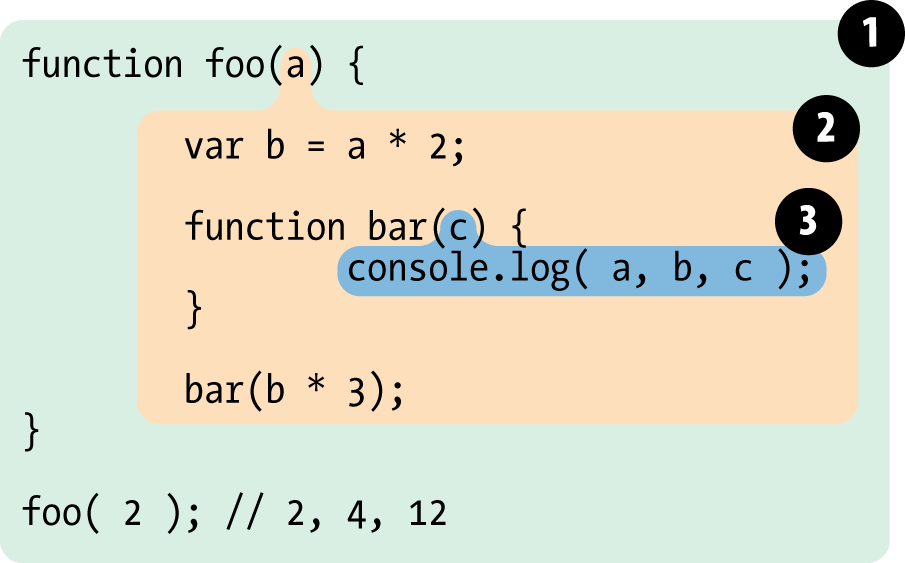
\includegraphics[keepaspectratio]{img/fig2.png}
\caption{Nested scope in source code (Simpson 2014)}
\label{fig:getify}
\end{figure}

The relation of nested scope to source code is illustrated by figure
\ref{fig:getify}. The \gls{function} \texttt{foo} is defined \emph{in}
the global scope (1) (see next section), and is therefore accessible
from all parts of this program. \texttt{foo} itself defines a new scope
(2) which includes the identifiers \texttt{a}, \texttt{b} and
\texttt{bar}. \texttt{bar} defines a new scope (3) within \texttt{foo},
declaring only the identifier \texttt{c}. As can be seen, the innermost
scope (3) has access to its own identifiers, as well as to the ones
defined in its ancestor scopes (2).

Figure \ref{fig:scopechain} shows the scope hierarchy for the source
code of listing \ref{lst:server} (see appendix). Assuming that, in a
given context, the anonymous function nested inside
\texttt{parseMarkdown()} is the active scope (marked in orange colour),
the figure shows its scope chain, consisting of the three scopes
\texttt{GLOBAL}, \texttt{parseMarkdown()}, and
\texttt{(anonymous function)}.

\begin{figure}[htbp]
\centering
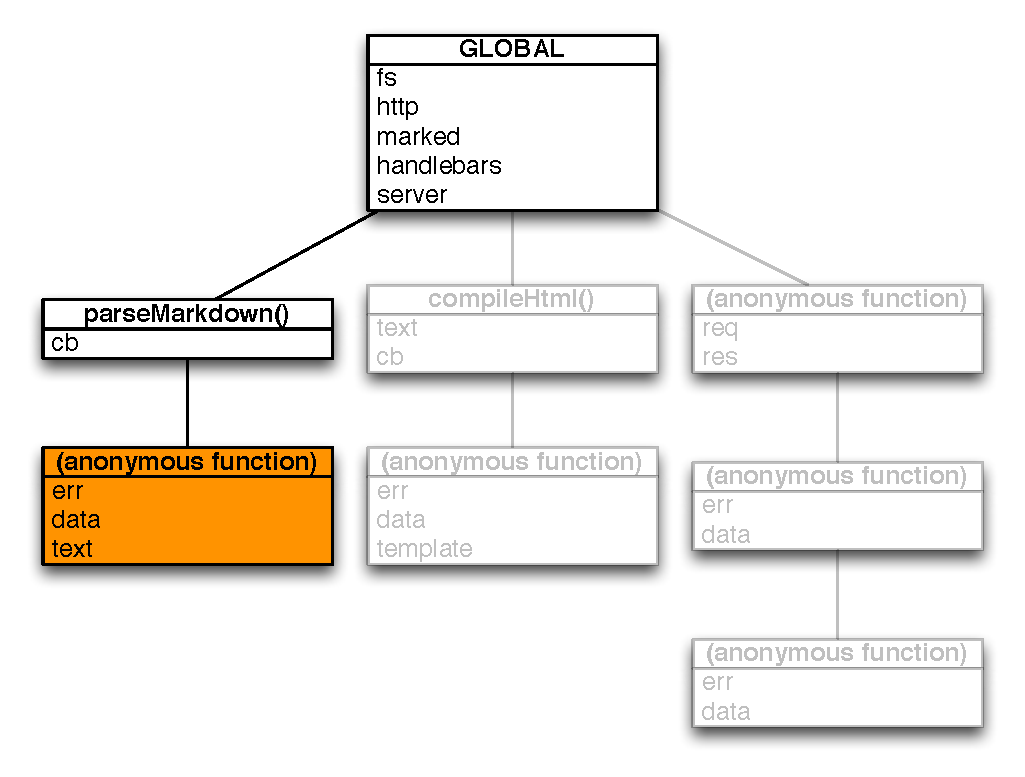
\includegraphics[keepaspectratio,width=0.7\textwidth]{img/scopechain.pdf}
\caption{Scope as hierarchical data structure; highlighted scope chain}
\label{fig:scopechain}
\end{figure}

\subsection{Scoping Models}\label{scoping-models}

As mentioned above, the rules for when a new scope is defined differ
depending on the programming language. Usually, a language implements
multiple of the following rules.

\begin{description}
\item[Global scope]
Variables that are accessible from \emph{any point} in the program are
in the global scope. The original BASIC programming language only
implemented global scope.
\item[Block scope]
Any logical block, often enclosed by curly brackets (\texttt{\{} and
\texttt{\}}), creates a new scope. This is the case in the C programming
language, amongst others.
\item[Function scope]
Any function definition defines a new scope. Parameters of the function
are part of this newly defined scope, as well as variables and functions
defined \emph{within} that function. JavaScript implements function
scope.
\item[Expression scope]
A variable’s scope is limited to a single expression. This useful for
very short-living, temporary variables. It is implemented by many
functional languages, for example Python and \gls{ecmascript} 6.
\end{description}

JavaScript, as of ECMAScript 5, implements only \emph{global} and
\emph{function} scope
models\footnote{There are exceptions through the keywords `with` and `except` and the function `eval`.}.
The run-time environment usually populates the global scope with several
objects and methods. The JavaScript engines in web browsers, for
instance, provide access to the \ac{dom} through the \texttt{document}
object.

\subsection{Common scoping problems}\label{common-scoping-problems}

The following are common phenomena that arise through scoping and may be
the cause of problems and misconceptions. Though being typical for
JavaScript, many of those problems can arise in other programming
languages, in the same or similar form, as well.

These phenomena can in most cases be either helpful or hindering, and
thus be desired or undesired. The goal of the concept developed in this
thesis is to make the developer recognize those phenomena during
author-time, and thus avoid misconceptions and reduce defects.

\begin{description}
\item[Hoisting]
is the implicit process, as done by the JavaScript engine, of moving
variable and function declarations „from where they appear in the flow
of the code to the top of the code“ \cite{getify}. By „code“,
\citename{getify} refers to the scope block. Any variable declaration
inside a scope block is hoisted to the top of the scope block.

\begin{verbatim}
        function foo() {
          a = 2;
          var a;
          console.log( a );
        }
\end{verbatim}

The above code is actually processed as:

\begin{verbatim}
        function foo() {
          var a;
          a = 2;
          console.log( a );
        }
\end{verbatim}

The variable declaration of \texttt{a} is moved, or „hoisted“, to the
top of the scope block of \texttt{foo}. Hoisting can impose unexpected
behaviour, especially when declaring variables of the same name in
nested scopes.
\item[Closure]
is a common phenomenon in JavaScript programs, and is widely used,
though being generally seen as hard to understand. Citing
\citename{getify}, closure is „when a function is able to remember and
access its lexical scope even when that function is executing outside
its lexical scope.“ \citeyear{getify} As functions are first-class
objects in JavaScript, they can be passed around like variables, for
example as asynchronous callback functions. A function can also return
another function. However, JavaScript works with \emph{lexical scope}
and, according to the nesting rules presented before, a function must
always have access to its ancestor scopes. Thus, when a function is
being returned or passed as a callback, an instance of the whole scope
chain is returned or passed along with the function. In other words, the
function „closes“ or „forms a closure“ over its ancestor scopes. In most
cases, this behaviour is desired. Anyway, it is important to recognize
closures as they may impact performance: the closed-over scopes have to
stay in memory as long as a reference to the closure exists. Closure may
also lead to unexpected behaviour, for example if a variable defined
outside of a closure is used inside of it (see
\citeasnoun*[Ch. 5]{getify} for examples).
\item[Shadowing]
is a consequence of nested scopes. If a variable (1) is defined in an
ancestor scope, and a new variable (2) of the same name is defined in a
descendant scope, the descendant scope has no access to (1). This is due
to the mechanism of variable lookup explained above. Variable (1) is
\emph{shadowed} by variable (2). As with most of the phenomenons listed
here, this can either be desired or unwanted behaviour. A good solution
to avoid shadowing is to choose different variable names throughout
nested scopes.
\item[Implicit variable declaration]
JavaScript allows for the creation of variables and object properties in
an implicit way (\emph{silently}). Instead of declaring a variable using
a \texttt{var} statement, they can as well just be used without prior
declaration, for example like this:

\begin{verbatim}
i = 3;
\end{verbatim}

Variables used without prior declaration are implicitly declared in the
\emph{global
scope}\footnote{ECMAScript 5’s \emph{strict mode} considers this an error.}.
As this is usually unwanted behaviour, it is considered good practice to
always declare variables explicitly. However, this problem is already
addressed by linters (see section \fullref{similar}).
\item[Lookup performance]
The variable lookup through scope chains, as described above, can have
an impact on the performance of an application. Each time a variable is
encountered, the JavaScript engine performs the lookup process,
navigating from the bottom of the scope chain upwards until it is found.
If a variable, which is defined in an ancestor scope (the global scope,
for example), is accessed within a deeply nested scope, the lookup
process slows down the execution of the program, as shown by
\citeasnoun{castorina}. He furthermore suggests to cache the variable in
a „closer“ scope, if possible.
\end{description}

Four of these five identified problems—\emph{hoisting}, \emph{closure},
\emph{shadowing}, and \emph{lookup performance}—need to be addressed by
the design concepts created in chapter \fullref{ideation} and prototyped
in chapter \fullref{design}. \emph{Implicit variable declaration},
however, is already addressed by linting tools and is therefore not in
focus of this design process.
